\section{Teknologibeskrivelse} \label{sec:teknologibeskrivelse}
Aktivitetsarmbånd bliver i stigende grad mere udbredt. Ifølge International Data Corporation er der sket en stigning i salget af aktivitetsarmbånd fra $11,8$ millioner enheder i første kvartal af 2015 til $19,7$ millioner i første kvartal af 2016 \citep{IDC2016}.

Det er fundet, at Fitbit udgør en stor andel af markedet for aktivitetsarmbånd og, at der fra første kvartal i 2015 til første kvartal i 2016, er sket en stigning i salget på $1$ million enheder \citep{IDC2016}.  
Fitbit Flex illustreres på \autoref{fig:fitbitflexarmbånd}. 

\begin{figure}[H]
	\centering
	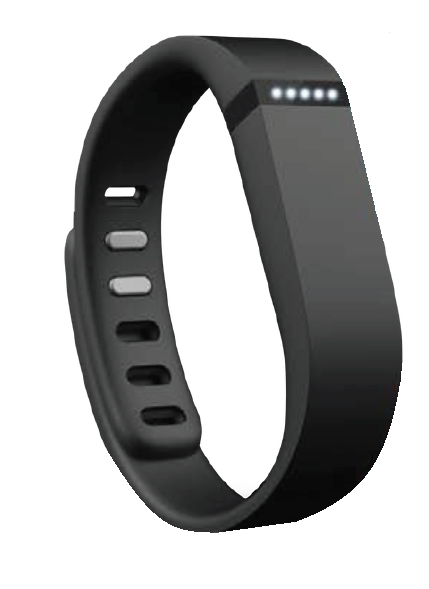
\includegraphics[width=0.3\textwidth]{figures/fitbitflex}
	\caption{Fitbit Flex armbånd med flex tracker \citep{fitbitflex}.}
	\label{fig:fitbitflexarmbånd}
\end{figure}

\noindent
Overordnet består Fitbit Flex med tilbehør af en flex tracker, opladerkabel, trådløs synkroniserings dongle og armbånd til flex tracker \citep{fitbitflex}. Disse kan ses af \autoref{fig:fitbitflexindhold}. 

\begin{figure}[H]
	\centering
	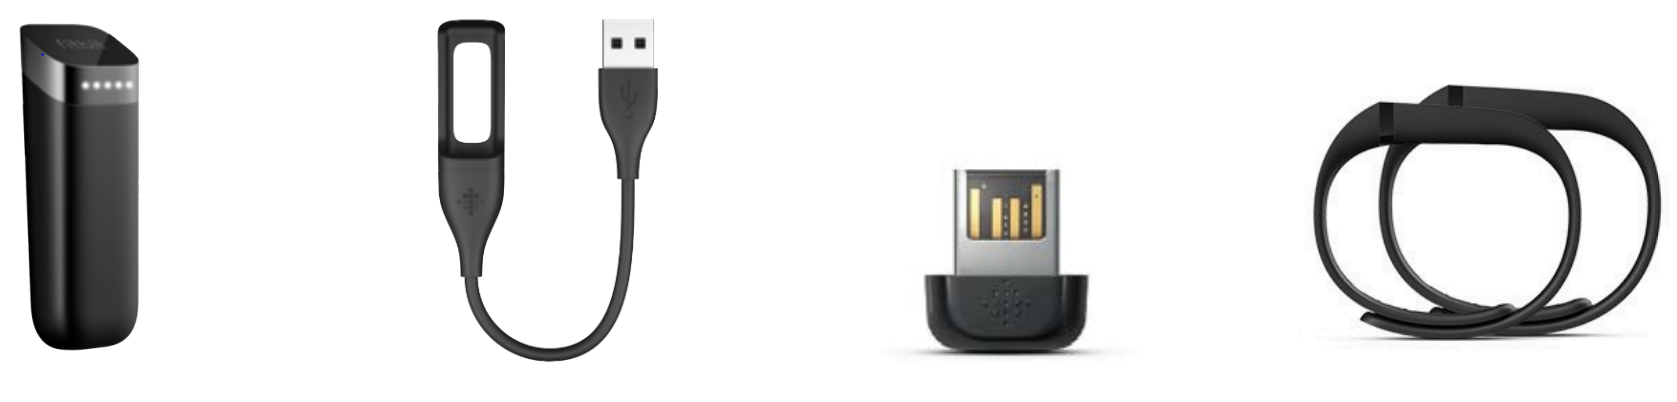
\includegraphics[width=0.6\textwidth]{figures/fitbitflexindhold}
	\caption{Fra venstre mod højre ses de forskellige dele af Fitbit Flex pakken, bestående af flex tracker, opladerkabel, trådløs synkroniserings dongle og armbånd \citep{fitbitflex}.}
	\label{fig:fitbitflexindhold}
\end{figure}

\noindent
Fitbit Flex er i stand til at måle antal minutter, brugeren er aktiv, længden samt kvaliteten af søvn og antal skridt. Af dette estimeres antal forbrændte kalorier og tilbagelagt afstand. 
Flex trackeren skal synkroniseres med en kompatibel enhed, hvis brugeren skal se den registrede aktivitet, da armbåndet kun besidder et display bestående af fem LEDer \citep{fitbitflex}. 

Synkronisering foregår trådløst ved brug af bluetooth low energy (BLE) og kan foregå mellem forskellige enheder såsom smartphone og computer. 
Synkronisering mellem flex tracker og computer kræver dog anvendelse af den trådløse synkroniserings dongle, der ses af \autoref{fig:fitbitflexindhold}.
Forudsætninger for, at data kan synkroniseres er, at en kompatibel enhed har den korrekte applikation installeret, hvor synkroniseringen ellers sker automatisk idet applikationen åbnes.  
Yderligere skal der oprettes en brugerkonto på \url{www.fitbit.com}, hvor brugeren oplyser personlige informationer: køn, alder, højde og vægt. Dette er nødvendigt i forhold til optimering af dataopsamling og estimering af forbrændte kalorier \citep{fitbitflex}.  

Gennem applikationen visualiseres den registrerede aktivitet, hvor brugeren har mulighed for at se data fra anvendelsesperioden. Data kan også observeres på Fitbits hjemmeside, hvor det er muligt at logge ind via brugerkontoen. 
Således ville alle i besiddelse af en given brugerkonto have adgang til den synkroniserede data, uden fysisk at have hverken bruger eller armbånd til stede. 
Til den daglige aktivitet har brugeren mulighed for at sætte bestemte mål til den fysiske aktivitet. Alt efter, hvilke mål brugeren sætter for sig selv, kan progressionen ses ud fra de fem LEDer på armbåndet ved, at brugeren trykker to gange på armbåndet \citep{fitbitflex}.   

Når ét af brugerens mål gennemføres, visualiseres dette ved, at de 5 LEDer blinker, og at armbåndet vibrerer. 
Fitbit Flex er ikke i stand til at visualisere armbåndets batteriniveau, og kan derfor kun ses via applikationen. 
Hukommelsen i flex trackeren tillader detaljeret data at blive lagret i perioder op til 7 dage og består af minut til minut målinger.  
Yderligere lagres summeringer af daglig aktivitet i op til 30 dage. 
Ved jævnlig synkronisering er det muligt for brugeren at bevare detaljeret data, da informationen tilknyttes brugerkontoen. 
Fitbit anbefaler én daglig synkronisering, dog er det ikke en nødvendighed \citep{fitbitflex}. 

\subsection{Hardware}
Fitbit Flex trackeren har forskellige hardware elementer, hvorfra trackeren signalerer og detekterer fysisk aktivitet. Hardwaren i trackeren udgøres af et display, batteri, en sensor og en motor \citep{fitbitflex}.
 
\subsubsection{Display} 
Flex trackeren er udstyret med fem LEDer, der ved forskellige operationstilstande, såsom alarm, aktivitet eller søvntracking, signalerer til brugeren. 
LEDerne kan fungere som indikator for progressionen i forhold til det brugerdefinerede fysiske mål for dagen. Hertil vil hver LED repræsentere en procentvis progression i intervaller af $20~\%$. Ved $73~\%$ progression af det daglige fysiske mål, vil de første tre LEDer lyse, og den fjerde vil blinke. Dette indikerer, at brugeren har nået $60~\%$ af målet, og at brugeren nu befinder sig mellem $60~\%$ og $80~\%$. 
Det samme gør sig gældende, når flex trackeren sættes til opladning. Her indikerer LEDerne, hvor langt armbåndet er fra fuld opladning \citep{fitbitflex}. 


\subsubsection{Sensor} 
Flex trackeren registrerer den fysiske aktivitet ved anvendelse af et 3-akses mikro elektro-mekanisk accelerometer, hvilket er den eneste sensor, som er implementeret i armbåndet. Et 3-akses accelerometer kan måle accelerationen i x-, y- og z-retning og kan give et udtryk for ændringerne i hastigheden \citep{ravi2005}. Ud fra algoritmer analyseres bevægelsesmønstre, hvorved der kan oplyses hvor mange skridt, der er foretaget under løb eller gang, samt den estimerede tilbagelagte afstand. 

\subsubsection{Motor}
Flex trackeren er udstyret med en vibrationsmotor, der aktiveres under forskellige funktioner, når armbåndet anvendes. Disse fungerer i sammenspil med displayet som et kommunikationsredskab for brugeren. Vibration aktiveres ved anvendelse af alarmfunktion, og ved aktivering eller deaktivering af sleep mode, samt når det daglige mål for fysisk aktivitet nås. 

\subsubsection{Batteri} 
Levetiden på Fitbit Flex' batteri er op til fem dage, afhængigt af, hvor ofte armbåndet synkroniseres for at visualisere progressionen.
Fitbit Flex indeholder et genopladeligt batteri, der oplades ved brug af det medfølgende kabel. Dette ses af \autoref{fig:fitbitflexindhold}. 

\subsection{Software}
Applikationen, som kan installeres på en smartphone, er brugerfladen, hvorfra den synkroniserede data formidles til brugeren. Beskrivelsen af brugerfladen er gjort ud fra anvendelse af applikationen og hjemmesiden som følge af, at Fitbit ikke har en konkret guide til den samlede software. I brugerfladen oplyses skridt, forbrændte kalorier med mere. 
Alt efter brugerens interesser, kan der også udfyldes informationer omkring indtaget kost ved brug af applikationen. Brugeren kan ud fra dette få et estimat af, hvor mange kalorier, denne har indtaget, hvortil dette kan sammenlignes med antal kalorier forbrændt. Anvendelsen af denne funktion er dog ikke en nødvendighed for anvendelsen af Fitbit Flex eller applikationen, dog kan dette give en praktiserende læge indblik i, om patienten overholder lægens anbefalinger for den hypertensive patient, både i forhold til kostvaner og fysisk aktivitet.

\begin{figure}[H]
	\centering
	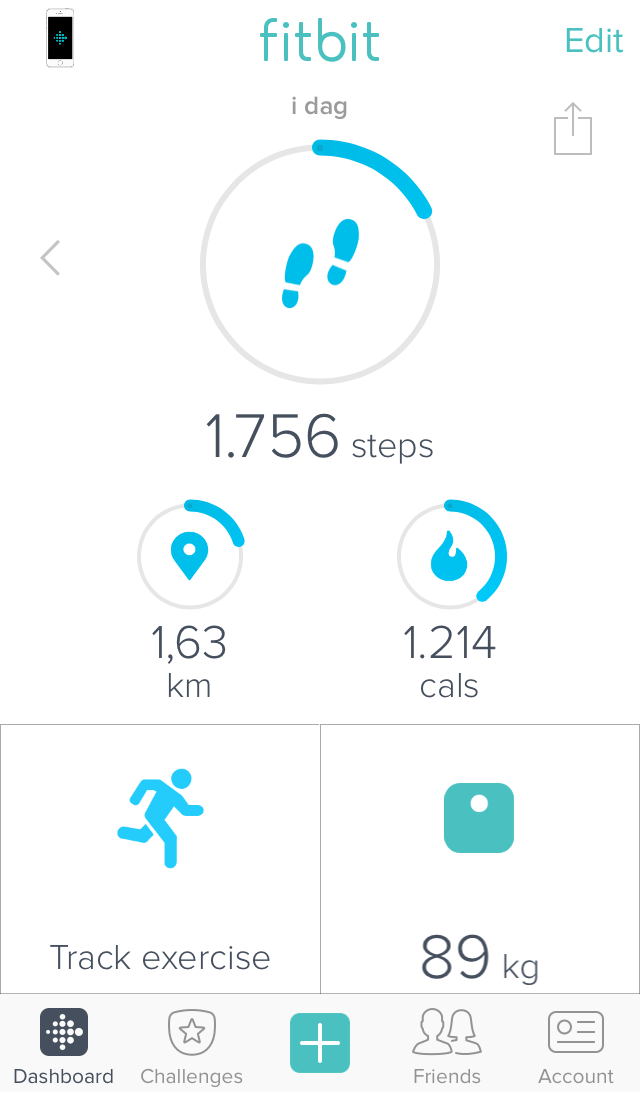
\includegraphics[width=0.45\textwidth]{figures/burgerfladeoversigt}
	\caption{Oversigt over fysisk aktivitet, der vises idet applikationen åbnes. Her ses blandt andet antal skridt taget, tilbagelagt afstand og kalorier forbrændt.}
	\label{fig:brugerfladeoversigt}
\end{figure}

\noindent
Af \autoref{fig:brugerfladeoversigt} ses en oversigt over den registrerede aktivitet, som var den målt gennem Fitbit Flex. Her ses antal skridt taget, tilbagelagt afstand og kalorier forbrændt. Af oversigten ses også, hvor langt brugeren er fra at opfylde de forskellige aktivitetsmål, disse er repræsenteret af den blå cirkel omkring de forskellige angivelser. 
I bunden ses fire forskellige oversigter, hvor der fra venstre mod højre ses 'Dashboard', 'Challenges', 'Friends' og 'Account'. Plus-tegnet i midten fungerer som en genvej til forskellige funktioner under de fire oversigter. 
'Dashboard' er den overordnede oversigt, som illustreres på \autoref{fig:brugerfladeoversigt}.
'Challenges' viser en oversigt over tilvalgte aktivitetsudfordringer, hvor brugeren har mulighed for at opstille udfordringer med venner samt andre brugere af applikationen. 
'Friends' giver brugeren et overblik over venner, der er tilføjet til applikationen. 
'Account' viser et overblik over, hvilken bruger, der er logget ind, og hvilken Fitbit enhed, der er tilsluttet applikationen. Yderligere kan der foretages ændringer af profil og mål for daglig fysisk aktivitet. 

En detaljeret oversigt over ydet aktivitet kan ses under den overordnede oversigt ved at trykke på de specifikke målinger. Ved at trykke på 'Steps' ses eksemplet, der fremgår af \autoref{fig:brugerfladesteps}.  

 % Kan ikke henvise til disse figurer.
\begin{figure}[H]
	\centering
	\begin{minipage}{0.48\textwidth}
		\centering
		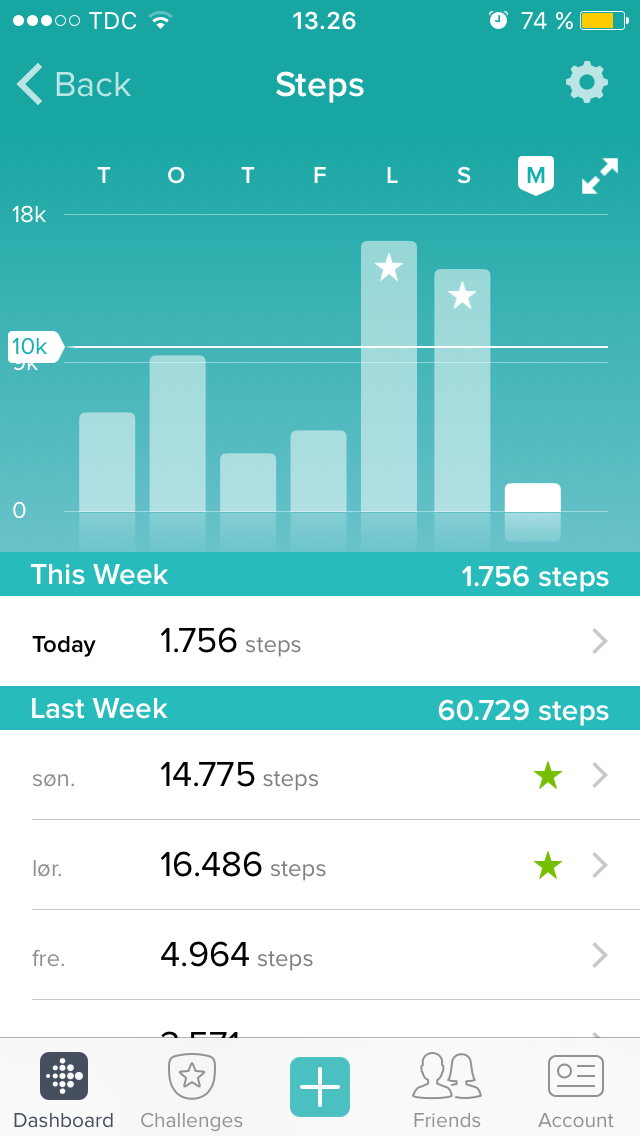
\includegraphics[width=0.8\linewidth]{figures/brugerfladesteps}
		\caption{Oversigt over skridt taget for den  forudgående uge delt op i ugens dage, som graf (øverst) og tabel (nederst).}
		\label{fig:brugerfladesteps}
	\end{minipage}%
	\hspace{3mm}
	\begin{minipage}{0.48\textwidth}
		\centering		
		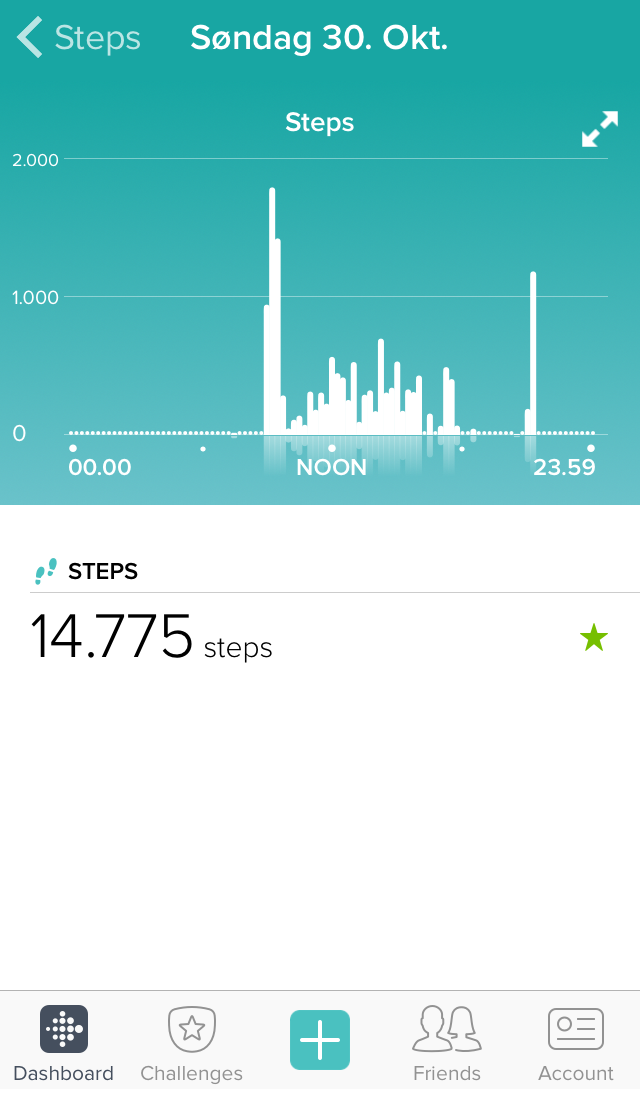
\includegraphics[width=0.8\linewidth]{figures/specifiksteps}
		\caption{Oversigt over skridt taget for én dag, som graf fordelt på døgnets timer (øverst) og i endeligt antal skridt (nederst).}
		 \label{fig:specifiksteps}
	\end{minipage}
\end{figure}

\noindent
Af \autoref{fig:brugerfladesteps} ses der øverst en graf over antal skridt taget inden for den sidste uge. Af grafen ses en hvid tværgående linje, der repræsenterer målet for antal skridt for dagen. Hertil ses, at dage, hvor målet er blevet opfyldt, markeres med en stjerne.

Under grafen ses en oversigt over antal skridt taget for de forhenværende dage, rækkende tilbage til den første anvendelsesdato. Heraf ses ligeledes at dagene, hvor målet nås, er indikeret med en stjerne. 

Ved at trykke på den givne dag eller en af de forhenværende dage, kan der ses en mere detaljeret oversigt over antal skridt taget i løbet af den pågældende dag. Dette ses af \autoref{fig:specifiksteps}, hvor det er muligt at se på, hvilke tider af dagen, brugeren er mest aktiv.  

\subsubsection{Brugerflade på nettet}

Det sociale aspekt af Fitbits brugerflade giver mulighed for at følge andre brugere, hvorved det er muligt at følge deres aktivitet gennem Fitbits hjemmeside. Afhængigt af privatindstillinger kan antal skridt, tilbagelagt afstand, søvnkvalitet, vægt og tid med forskellige aktivitetsniveauer ses på brugerens profil. Her er det muligt at se de førnævnte detaljer om brugeren for de seneste $30$ dage, som vist på \autoref{fig:netbruger}.

\begin{figure}[H]
	\centering
	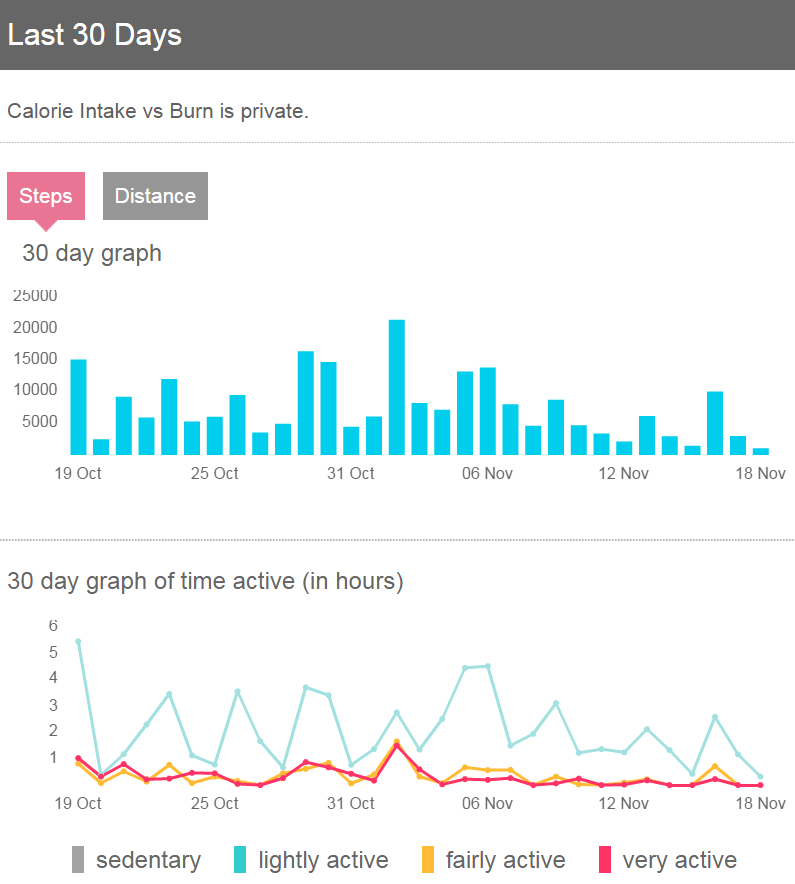
\includegraphics[width=0.45\textwidth]{figures/Netbruger}
	\caption{Oversigt over fysisk aktivitet hos en bruger, som set på Fitbits hjemmeside}
	\label{fig:netbruger}
\end{figure}

\noindent
Ved at holde markøren over forskellige områder af graferne og søjlerne på \autoref{fig:netbruger}, er det muligt at se præcise tal for aktiviteten. Søjlerne vist øverst på figuren, er antallet af skridt brugeren har taget, og kan med knappen 'Distance' ændres således, at den tilbagelagte afstand vises i stedet. Graferne nederst på figuren viser antal timer med henholdsvis let, middel og intens aktivitet, hvorved det er muligt at se, hvor mange aktive timer, brugeren har i løbet af dagen. 

\subsection{Brugertilpasning} \label{sec:brugertilpasning}
Der er forskellige muligheder for at tilpasse armbåndet optimalt til den givne bruger. Heriblandt er der mulighed for at udskifte armbåndet til andre længder, og at tilpasse skridtlængden til den enkelte bruger. Foruden dette egner armbåndet sig til at blive brugt under forskellige vejrforhold, da Fitbit Flex er vandafvisende. 

%{Forskellige Fitbit Flex armbånd}
%Brugeren har mulighed for at vælge armbånd i to forskellige længder. Dette tillader muligheden for bedre tilpasning omkring håndleddet. Armbåndene kan ligeledes fås i forskellige farver.

\subsubsection{Kalibrering af skridtlængde}
Applikationen vurderer som standard brugerens skridtlængde ud fra de angivne oplysninger omkring brugerens højde ved oprettelsen af brugerkontoen. Brugeren har dog mulighed for at kalibrere denne værdi i tilfælde af, at brugeren opdager uoverensstemmelse mellem registreret tilbagelagt afstand og reel tilbagelagt afstand. Brugeren kan under indstillinger i applikationen ændre den prædefinerede skridtlængde til en mere passende værdi. Fitbit oplyser på deres supporthjemmeside guidelines for, hvordan brugeren selv kan udregne en individuelt tilpasset skridtlængde.   

\begin{comment}
Hvad består teknologien af?
Hvor udbredt er teknologien?
Hvordan tilpasses teknologien den enkelte person?
Levetid for teknologien?
Hvilke muligheder er der for lagring og videregivelse af information til en læge?
\end{comment}
